\documentclass[1p]{elsarticle_modified}
%\bibliographystyle{elsarticle-num}

%\usepackage[colorlinks]{hyperref}
%\usepackage{abbrmath_seonhwa} %\Abb, \Ascr, \Acal ,\Abf, \Afrak
\usepackage{amsfonts}
\usepackage{amssymb}
\usepackage{amsmath}
\usepackage{amsthm}
\usepackage{scalefnt}
\usepackage{amsbsy}
\usepackage{kotex}
\usepackage{caption}
\usepackage{subfig}
\usepackage{color}
\usepackage{graphicx}
\usepackage{xcolor} %% white, black, red, green, blue, cyan, magenta, yellow
\usepackage{float}
\usepackage{setspace}
\usepackage{hyperref}

\usepackage{tikz}
\usetikzlibrary{arrows}

\usepackage{multirow}
\usepackage{array} % fixed length table
\usepackage{hhline}

%%%%%%%%%%%%%%%%%%%%%
\makeatletter
\renewcommand*\env@matrix[1][\arraystretch]{%
	\edef\arraystretch{#1}%
	\hskip -\arraycolsep
	\let\@ifnextchar\new@ifnextchar
	\array{*\c@MaxMatrixCols c}}
\makeatother %https://tex.stackexchange.com/questions/14071/how-can-i-increase-the-line-spacing-in-a-matrix
%%%%%%%%%%%%%%%

\usepackage[normalem]{ulem}

\newcommand{\msout}[1]{\ifmmode\text{\sout{\ensuremath{#1}}}\else\sout{#1}\fi}
%SOURCE: \msout is \stkout macro in https://tex.stackexchange.com/questions/20609/strikeout-in-math-mode

\newcommand{\cancel}[1]{
	\ifmmode
	{\color{red}\msout{#1}}
	\else
	{\color{red}\sout{#1}}
	\fi
}

\newcommand{\add}[1]{
	{\color{blue}\uwave{#1}}
}

\newcommand{\replace}[2]{
	\ifmmode
	{\color{red}\msout{#1}}{\color{blue}\uwave{#2}}
	\else
	{\color{red}\sout{#1}}{\color{blue}\uwave{#2}}
	\fi
}

\newcommand{\Sol}{\mathcal{S}} %segment
\newcommand{\D}{D} %diagram
\newcommand{\A}{\mathcal{A}} %arc


%%%%%%%%%%%%%%%%%%%%%%%%%%%%%5 test

\def\sl{\operatorname{\textup{SL}}(2,\Cbb)}
\def\psl{\operatorname{\textup{PSL}}(2,\Cbb)}
\def\quan{\mkern 1mu \triangleright \mkern 1mu}

\theoremstyle{definition}
\newtheorem{thm}{Theorem}[section]
\newtheorem{prop}[thm]{Proposition}
\newtheorem{lem}[thm]{Lemma}
\newtheorem{ques}[thm]{Question}
\newtheorem{cor}[thm]{Corollary}
\newtheorem{defn}[thm]{Definition}
\newtheorem{exam}[thm]{Example}
\newtheorem{rmk}[thm]{Remark}
\newtheorem{alg}[thm]{Algorithm}

\newcommand{\I}{\sqrt{-1}}
\begin{document}

%\begin{frontmatter}
%
%\title{Boundary parabolic representations of knots up to 8 crossings}
%
%%% Group authors per affiliation:
%\author{Yunhi Cho} 
%\address{Department of Mathematics, University of Seoul, Seoul, Korea}
%\ead{yhcho@uos.ac.kr}
%
%
%\author{Seonhwa Kim} %\fnref{s_kim}}
%\address{Center for Geometry and Physics, Institute for Basic Science, Pohang, 37673, Korea}
%\ead{ryeona17@ibs.re.kr}
%
%\author{Hyuk Kim}
%\address{Department of Mathematical Sciences, Seoul National University, Seoul 08826, Korea}
%\ead{hyukkim@snu.ac.kr}
%
%\author{Seokbeom Yoon}
%\address{Department of Mathematical Sciences, Seoul National University, Seoul, 08826,  Korea}
%\ead{sbyoon15@snu.ac.kr}
%
%\begin{abstract}
%We find all boundary parabolic representation of knots up to 8 crossings.
%
%\end{abstract}
%\begin{keyword}
%    \MSC[2010] 57M25 
%\end{keyword}
%
%\end{frontmatter}

%\linenumbers
%\tableofcontents
%
\newcommand\colored[1]{\textcolor{white}{\rule[-0.35ex]{0.8em}{1.4ex}}\kern-0.8em\color{red} #1}%
%\newcommand\colored[1]{\textcolor{white}{ #1}\kern-2.17ex	\textcolor{white}{ #1}\kern-1.81ex	\textcolor{white}{ #1}\kern-2.15ex\color{red}#1	}

{\Large $\underline{12n_{0550}~(K12n_{0550})}$}

\setlength{\tabcolsep}{10pt}
\renewcommand{\arraystretch}{1.6}
\vspace{1cm}\begin{tabular}{m{100pt}>{\centering\arraybackslash}m{274pt}}
\multirow{5}{120pt}{
	\centering
	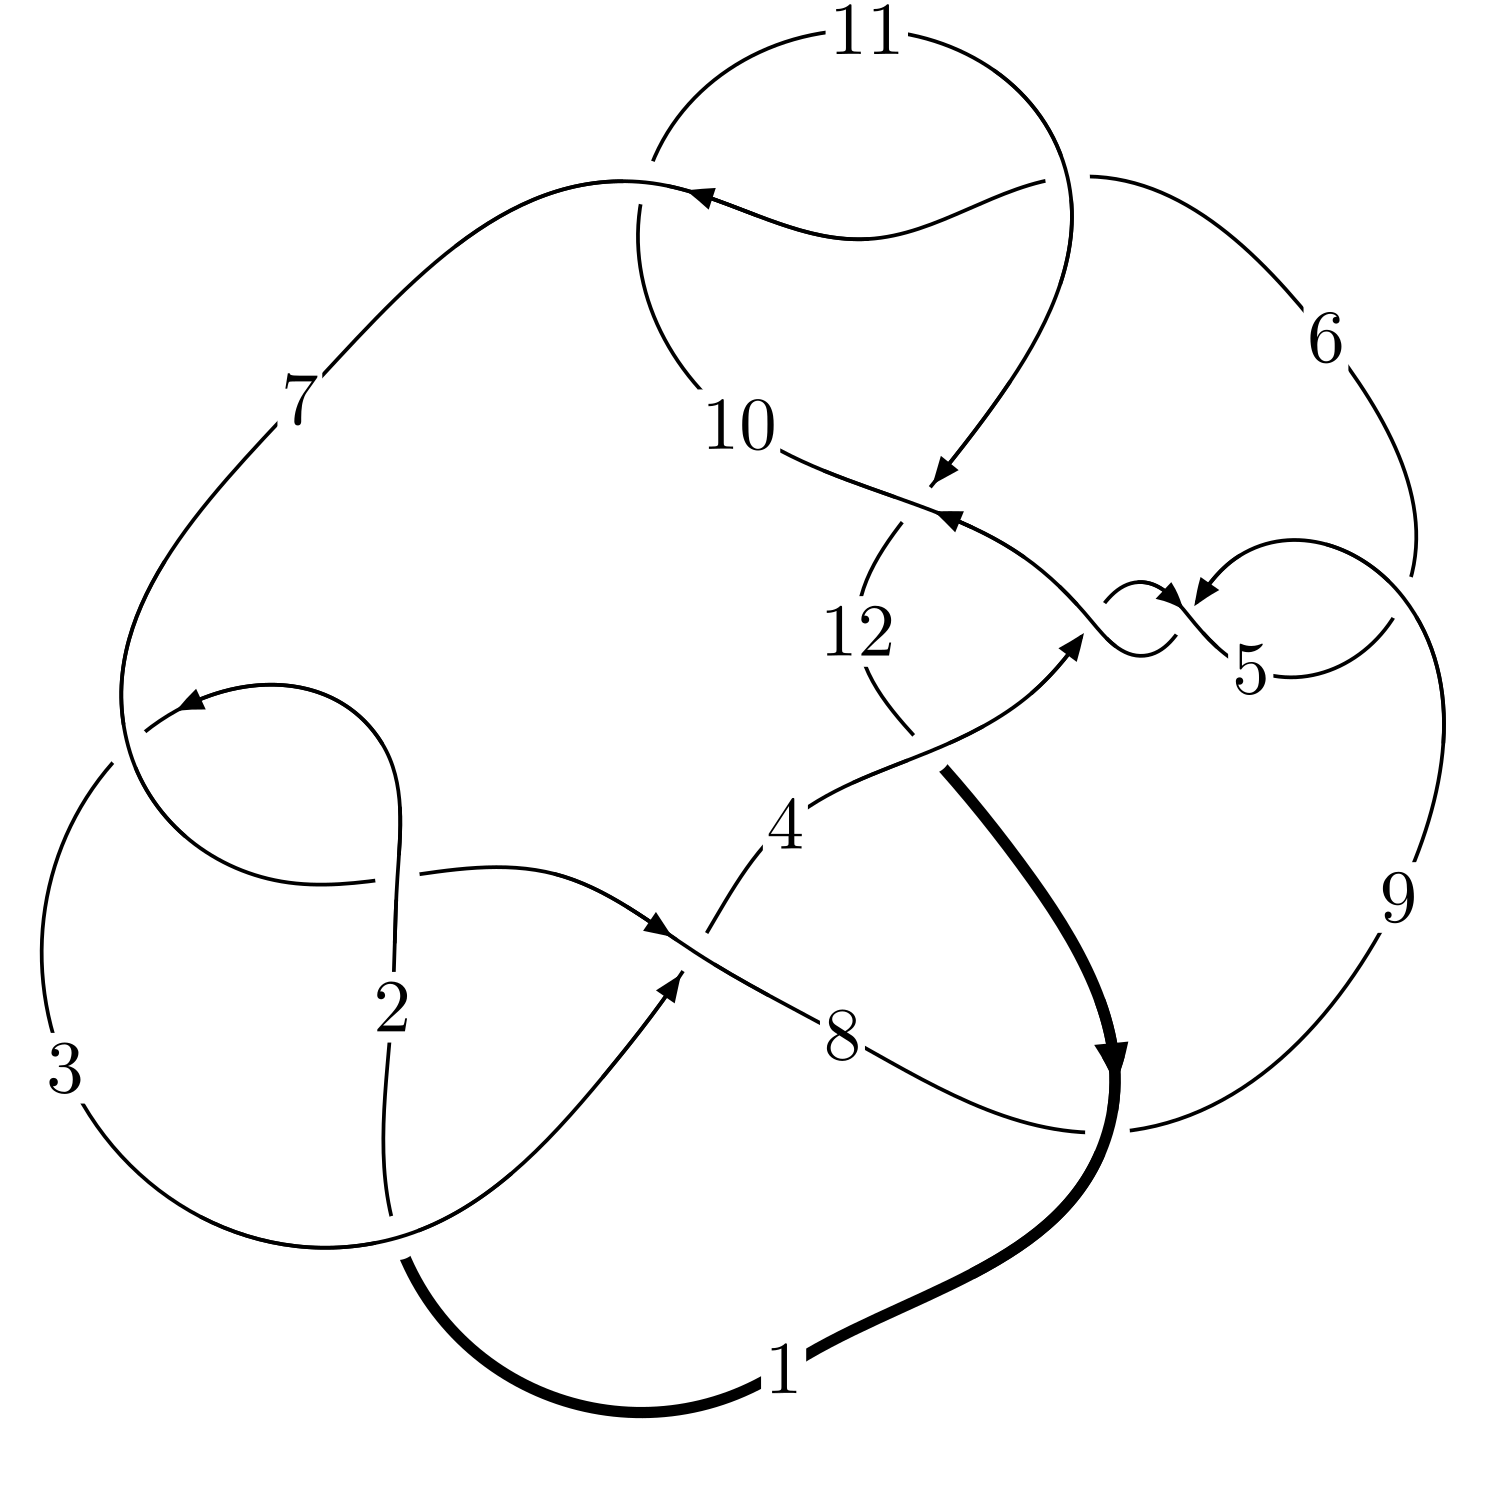
\includegraphics[width=112pt]{../../../GIT/diagram.site/Diagrams/png/2639_12n_0550.png}\\
\ \ \ A knot diagram\footnotemark}&
\allowdisplaybreaks
\textbf{Linearized knot diagam} \\
\cline{2-2}
 &
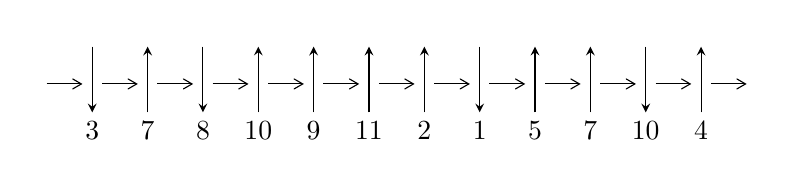
\begin{tikzpicture}[x=20pt, y=17pt]
	% nodes
	\node (C0) at (0, 0) {};
	\node (C1) at (1, 0) {};
	\node (C1U) at (1, +1) {};
	\node (C1D) at (1, -1) {3};

	\node (C2) at (2, 0) {};
	\node (C2U) at (2, +1) {};
	\node (C2D) at (2, -1) {7};

	\node (C3) at (3, 0) {};
	\node (C3U) at (3, +1) {};
	\node (C3D) at (3, -1) {8};

	\node (C4) at (4, 0) {};
	\node (C4U) at (4, +1) {};
	\node (C4D) at (4, -1) {10};

	\node (C5) at (5, 0) {};
	\node (C5U) at (5, +1) {};
	\node (C5D) at (5, -1) {9};

	\node (C6) at (6, 0) {};
	\node (C6U) at (6, +1) {};
	\node (C6D) at (6, -1) {11};

	\node (C7) at (7, 0) {};
	\node (C7U) at (7, +1) {};
	\node (C7D) at (7, -1) {2};

	\node (C8) at (8, 0) {};
	\node (C8U) at (8, +1) {};
	\node (C8D) at (8, -1) {1};

	\node (C9) at (9, 0) {};
	\node (C9U) at (9, +1) {};
	\node (C9D) at (9, -1) {5};

	\node (C10) at (10, 0) {};
	\node (C10U) at (10, +1) {};
	\node (C10D) at (10, -1) {7};

	\node (C11) at (11, 0) {};
	\node (C11U) at (11, +1) {};
	\node (C11D) at (11, -1) {10};

	\node (C12) at (12, 0) {};
	\node (C12U) at (12, +1) {};
	\node (C12D) at (12, -1) {4};
	\node (C13) at (13, 0) {};

	% arrows
	\draw[->,>={angle 60}]
	(C0) edge (C1) (C1) edge (C2) (C2) edge (C3) (C3) edge (C4) (C4) edge (C5) (C5) edge (C6) (C6) edge (C7) (C7) edge (C8) (C8) edge (C9) (C9) edge (C10) (C10) edge (C11) (C11) edge (C12) (C12) edge (C13) ;	\draw[->,>=stealth]
	(C1U) edge (C1D) (C2D) edge (C2U) (C3U) edge (C3D) (C4D) edge (C4U) (C5D) edge (C5U) (C6D) edge (C6U) (C7D) edge (C7U) (C8U) edge (C8D) (C9D) edge (C9U) (C10D) edge (C10U) (C11U) edge (C11D) (C12D) edge (C12U) ;
	\end{tikzpicture} \\
\hhline{~~} \\& 
\textbf{Solving Sequence} \\ \cline{2-2} 
 &
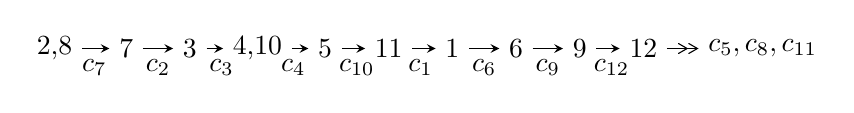
\begin{tikzpicture}[x=23pt, y=7pt]
	% node
	\node (A0) at (-1/8, 0) {2,8};
	\node (A1) at (1, 0) {7};
	\node (A2) at (2, 0) {3};
	\node (A3) at (49/16, 0) {4,10};
	\node (A4) at (33/8, 0) {5};
	\node (A5) at (41/8, 0) {11};
	\node (A6) at (49/8, 0) {1};
	\node (A7) at (57/8, 0) {6};
	\node (A8) at (65/8, 0) {9};
	\node (A9) at (73/8, 0) {12};
	\node (C1) at (1/2, -1) {$c_{7}$};
	\node (C2) at (3/2, -1) {$c_{2}$};
	\node (C3) at (5/2, -1) {$c_{3}$};
	\node (C4) at (29/8, -1) {$c_{4}$};
	\node (C5) at (37/8, -1) {$c_{10}$};
	\node (C6) at (45/8, -1) {$c_{1}$};
	\node (C7) at (53/8, -1) {$c_{6}$};
	\node (C8) at (61/8, -1) {$c_{9}$};
	\node (C9) at (69/8, -1) {$c_{12}$};
	\node (A10) at (11, 0) {$c_{5},c_{8},c_{11}$};

	% edge
	\draw[->,>=stealth]	
	(A0) edge (A1) (A1) edge (A2) (A2) edge (A3) (A3) edge (A4) (A4) edge (A5) (A5) edge (A6) (A6) edge (A7) (A7) edge (A8) (A8) edge (A9) ;
	\draw[->>,>={angle 60}]	
	(A9) edge (A10);
\end{tikzpicture} \\ 

\end{tabular} \\

\footnotetext{
The image of knot diagram is generated by the software ``\textbf{Draw programme}" developed by Andrew Bartholomew(\url{http://www.layer8.co.uk/maths/draw/index.htm\#Running-draw}), where we modified some parts for our purpose(\url{https://github.com/CATsTAILs/LinksPainter}).
}\phantom \\ \newline 
\centering \textbf{Ideals for irreducible components\footnotemark of $X_{\text{par}}$} 
 
\begin{align*}
I^u_{1}&=\langle 
u^{16}-3 u^{15}+\cdots+b+3,\;-3 u^{17}+7 u^{16}+\cdots+2 a+1,\;u^{18}-3 u^{17}+\cdots-5 u+2\rangle \\
I^u_{2}&=\langle 
- u^{10}-2 u^8-3 u^6- u^5-2 u^4- u^3- u^2+b- u-1,\\
\phantom{I^u_{2}}&\phantom{= \langle  }u^{11}+u^{10}+2 u^9+2 u^8+3 u^7+3 u^6+2 u^5+u^4+u^3+a+u,\;u^{12}+3 u^{10}+5 u^8+4 u^6+2 u^4+u^2+1\rangle \\
I^u_{3}&=\langle 
- u^4 a-2 u^2 a+u^3+a u+b- a+u-1,\;u^3 a+2 u^2 a+3 u^3+a^2+2 a u+3 u^2+2 a+u+1,\\
\phantom{I^u_{3}}&\phantom{= \langle  }u^5+u^4+2 u^3+u^2+u+1\rangle \\
\\
\end{align*}
\raggedright * 3 irreducible components of $\dim_{\mathbb{C}}=0$, with total 40 representations.\\
\footnotetext{All coefficients of polynomials are rational numbers. But the coefficients are sometimes approximated in decimal forms when there is not enough margin.}
\newpage
\renewcommand{\arraystretch}{1}
\centering \section*{I. $I^u_{1}= \langle u^{16}-3 u^{15}+\cdots+b+3,\;-3 u^{17}+7 u^{16}+\cdots+2 a+1,\;u^{18}-3 u^{17}+\cdots-5 u+2 \rangle$}
\flushleft \textbf{(i) Arc colorings}\\
\begin{tabular}{m{7pt} m{180pt} m{7pt} m{180pt} }
\flushright $a_{2}=$&$\begin{pmatrix}0\\u\end{pmatrix}$ \\
\flushright $a_{8}=$&$\begin{pmatrix}1\\0\end{pmatrix}$ \\
\flushright $a_{7}=$&$\begin{pmatrix}1\\u^2\end{pmatrix}$ \\
\flushright $a_{3}=$&$\begin{pmatrix}u\\u^3+u\end{pmatrix}$ \\
\flushright $a_{4}=$&$\begin{pmatrix}- u^3\\u^3+u\end{pmatrix}$ \\
\flushright $a_{10}=$&$\begin{pmatrix}\frac{3}{2} u^{17}-\frac{7}{2} u^{16}+\cdots+\frac{7}{2} u-\frac{1}{2}\\- u^{16}+3 u^{15}+\cdots+4 u-3\end{pmatrix}$ \\
\flushright $a_{5}=$&$\begin{pmatrix}-\frac{1}{2} u^{17}+\frac{3}{2} u^{16}+\cdots-\frac{3}{2} u+\frac{1}{2}\\u^{17}-2 u^{16}+\cdots+3 u-1\end{pmatrix}$ \\
\flushright $a_{11}=$&$\begin{pmatrix}\frac{5}{2} u^{17}-\frac{11}{2} u^{16}+\cdots+\frac{11}{2} u-\frac{3}{2}\\-2 u^{16}+5 u^{15}+\cdots+7 u-5\end{pmatrix}$ \\
\flushright $a_{1}=$&$\begin{pmatrix}u^3\\u^5+u^3+u\end{pmatrix}$ \\
\flushright $a_{6}=$&$\begin{pmatrix}-\frac{1}{2} u^{17}+\frac{3}{2} u^{16}+\cdots-\frac{1}{2} u+\frac{1}{2}\\2 u^{17}-3 u^{16}+\cdots+2 u-1\end{pmatrix}$ \\
\flushright $a_{9}=$&$\begin{pmatrix}u^8+u^6+u^4+1\\u^{10}+2 u^8+3 u^6+2 u^4+u^2\end{pmatrix}$ \\
\flushright $a_{12}=$&$\begin{pmatrix}- u^{11}-2 u^9-2 u^7+u^3\\u^{11}+3 u^9+4 u^7+3 u^5+u^3+u\end{pmatrix}$\\&\end{tabular}
\flushleft \textbf{(ii) Obstruction class $= -1$}\\~\\
\flushleft \textbf{(iii) Cusp Shapes $= -2 u^{17}+6 u^{16}-12 u^{15}+22 u^{14}-24 u^{13}+40 u^{12}-34 u^{11}+46 u^{10}-32 u^9+26 u^8-22 u^7+6 u^6+2 u^5-10 u^4+16 u^3+2 u^2+2 u+2$}\\~\\
\newpage\renewcommand{\arraystretch}{1}
\flushleft \textbf{(iv) u-Polynomials at the component}\newline \\
\begin{tabular}{m{50pt}|m{274pt}}
Crossings & \hspace{64pt}u-Polynomials at each crossing \\
\hline $$\begin{aligned}c_{1}\end{aligned}$$&$\begin{aligned}
&u^{18}+9 u^{17}+\cdots+3 u+4
\end{aligned}$\\
\hline $$\begin{aligned}c_{2},c_{7}\end{aligned}$$&$\begin{aligned}
&u^{18}+3 u^{17}+\cdots+5 u+2
\end{aligned}$\\
\hline $$\begin{aligned}c_{3}\end{aligned}$$&$\begin{aligned}
&u^{18}-3 u^{17}+\cdots-123 u+34
\end{aligned}$\\
\hline $$\begin{aligned}c_{4},c_{5},c_{6}\\c_{9},c_{10}\end{aligned}$$&$\begin{aligned}
&u^{18}+17 u^{16}+\cdots+6 u^2+1
\end{aligned}$\\
\hline $$\begin{aligned}c_{8}\end{aligned}$$&$\begin{aligned}
&u^{18}+15 u^{17}+\cdots+1169 u+266
\end{aligned}$\\
\hline $$\begin{aligned}c_{11}\end{aligned}$$&$\begin{aligned}
&u^{18}+34 u^{17}+\cdots+12 u+1
\end{aligned}$\\
\hline $$\begin{aligned}c_{12}\end{aligned}$$&$\begin{aligned}
&u^{18}+u^{17}+\cdots+265 u+160
\end{aligned}$\\
\hline
\end{tabular}\\~\\
\newpage\renewcommand{\arraystretch}{1}
\flushleft \textbf{(v) Riley Polynomials at the component}\newline \\
\begin{tabular}{m{50pt}|m{274pt}}
Crossings & \hspace{64pt}Riley Polynomials at each crossing \\
\hline $$\begin{aligned}c_{1}\end{aligned}$$&$\begin{aligned}
&y^{18}+y^{17}+\cdots+191 y+16
\end{aligned}$\\
\hline $$\begin{aligned}c_{2},c_{7}\end{aligned}$$&$\begin{aligned}
&y^{18}+9 y^{17}+\cdots+3 y+4
\end{aligned}$\\
\hline $$\begin{aligned}c_{3}\end{aligned}$$&$\begin{aligned}
&y^{18}-7 y^{17}+\cdots-3909 y+1156
\end{aligned}$\\
\hline $$\begin{aligned}c_{4},c_{5},c_{6}\\c_{9},c_{10}\end{aligned}$$&$\begin{aligned}
&y^{18}+34 y^{17}+\cdots+12 y+1
\end{aligned}$\\
\hline $$\begin{aligned}c_{8}\end{aligned}$$&$\begin{aligned}
&y^{18}-3 y^{17}+\cdots+155491 y+70756
\end{aligned}$\\
\hline $$\begin{aligned}c_{11}\end{aligned}$$&$\begin{aligned}
&y^{18}-126 y^{17}+\cdots+16 y+1
\end{aligned}$\\
\hline $$\begin{aligned}c_{12}\end{aligned}$$&$\begin{aligned}
&y^{18}+85 y^{17}+\cdots-550545 y+25600
\end{aligned}$\\
\hline
\end{tabular}\\~\\
\newpage\flushleft \textbf{(vi) Complex Volumes and Cusp Shapes}
$$\begin{array}{c|c|c}  
\text{Solutions to }I^u_{1}& \I (\text{vol} + \sqrt{-1}CS) & \text{Cusp shape}\\
 \hline 
\begin{aligned}
u &= \phantom{-}0.900621 + 0.268664 I \\
a &= -0.729720 + 0.016572 I \\
b &= -0.20830 - 2.38570 I\end{aligned}
 & -17.8823 - 5.8715 I & \phantom{-}1.17869 + 1.87367 I \\ \hline\begin{aligned}
u &= \phantom{-}0.900621 - 0.268664 I \\
a &= -0.729720 - 0.016572 I \\
b &= -0.20830 + 2.38570 I\end{aligned}
 & -17.8823 + 5.8715 I & \phantom{-}1.17869 - 1.87367 I \\ \hline\begin{aligned}
u &= \phantom{-}0.297755 + 1.056830 I \\
a &= \phantom{-}0.151471 - 1.118820 I \\
b &= \phantom{-}0.648988 + 0.730249 I\end{aligned}
 & -3.32385 + 0.53851 I & -1.31320 + 1.23447 I \\ \hline\begin{aligned}
u &= \phantom{-}0.297755 - 1.056830 I \\
a &= \phantom{-}0.151471 + 1.118820 I \\
b &= \phantom{-}0.648988 - 0.730249 I\end{aligned}
 & -3.32385 - 0.53851 I & -1.31320 - 1.23447 I \\ \hline\begin{aligned}
u &= -0.750892 + 0.811110 I \\
a &= -1.272950 + 0.346188 I \\
b &= \phantom{-}0.598966 - 0.460694 I\end{aligned}
 & -14.5019 - 2.7975 I & \phantom{-}1.40873 + 2.65752 I \\ \hline\begin{aligned}
u &= -0.750892 - 0.811110 I \\
a &= -1.272950 - 0.346188 I \\
b &= \phantom{-}0.598966 + 0.460694 I\end{aligned}
 & -14.5019 + 2.7975 I & \phantom{-}1.40873 - 2.65752 I \\ \hline\begin{aligned}
u &= -0.482590 + 1.071550 I \\
a &= \phantom{-}0.264991 - 0.374329 I \\
b &= -0.027718 + 0.293336 I\end{aligned}
 & -0.95248 - 3.40681 I & \phantom{-}4.19440 + 2.15670 I \\ \hline\begin{aligned}
u &= -0.482590 - 1.071550 I \\
a &= \phantom{-}0.264991 + 0.374329 I \\
b &= -0.027718 - 0.293336 I\end{aligned}
 & -0.95248 + 3.40681 I & \phantom{-}4.19440 - 2.15670 I \\ \hline\begin{aligned}
u &= \phantom{-}0.541968 + 1.089520 I \\
a &= -0.848196 + 0.994100 I \\
b &= -0.205313 - 1.329710 I\end{aligned}
 & -1.65747 + 6.51690 I & \phantom{-}2.73570 - 9.24962 I \\ \hline\begin{aligned}
u &= \phantom{-}0.541968 - 1.089520 I \\
a &= -0.848196 - 0.994100 I \\
b &= -0.205313 + 1.329710 I\end{aligned}
 & -1.65747 - 6.51690 I & \phantom{-}2.73570 + 9.24962 I\\
 \hline 
 \end{array}$$\newpage$$\begin{array}{c|c|c}  
\text{Solutions to }I^u_{1}& \I (\text{vol} + \sqrt{-1}CS) & \text{Cusp shape}\\
 \hline 
\begin{aligned}
u &= \phantom{-}0.643322 + 0.355418 I \\
a &= \phantom{-}0.486969 + 0.304277 I \\
b &= -0.228450 + 0.806417 I\end{aligned}
 & \phantom{-}0.44494 - 1.87013 I & \phantom{-}6.06834 + 5.46541 I \\ \hline\begin{aligned}
u &= \phantom{-}0.643322 - 0.355418 I \\
a &= \phantom{-}0.486969 - 0.304277 I \\
b &= -0.228450 - 0.806417 I\end{aligned}
 & \phantom{-}0.44494 + 1.87013 I & \phantom{-}6.06834 - 5.46541 I \\ \hline\begin{aligned}
u &= \phantom{-}0.266121 + 1.276470 I \\
a &= -0.55947 + 2.38028 I \\
b &= -1.03140 - 1.90393 I\end{aligned}
 & \phantom{-}16.5141 - 2.0953 I & -3.38488 - 0.11711 I \\ \hline\begin{aligned}
u &= \phantom{-}0.266121 - 1.276470 I \\
a &= -0.55947 - 2.38028 I \\
b &= -1.03140 + 1.90393 I\end{aligned}
 & \phantom{-}16.5141 + 2.0953 I & -3.38488 + 0.11711 I \\ \hline\begin{aligned}
u &= -0.504699 + 0.453241 I \\
a &= \phantom{-}0.598131 + 0.161265 I \\
b &= -0.263286 + 0.046770 I\end{aligned}
 & \phantom{-}0.920321 - 0.679889 I & \phantom{-}8.59008 + 5.05445 I \\ \hline\begin{aligned}
u &= -0.504699 - 0.453241 I \\
a &= \phantom{-}0.598131 - 0.161265 I \\
b &= -0.263286 - 0.046770 I\end{aligned}
 & \phantom{-}0.920321 + 0.679889 I & \phantom{-}8.59008 - 5.05445 I \\ \hline\begin{aligned}
u &= \phantom{-}0.588394 + 1.196870 I \\
a &= \phantom{-}2.15878 - 1.76754 I \\
b &= -0.28348 + 2.92630 I\end{aligned}
 & \phantom{-}18.7937 + 11.3151 I & -1.47787 - 5.35681 I \\ \hline\begin{aligned}
u &= \phantom{-}0.588394 - 1.196870 I \\
a &= \phantom{-}2.15878 + 1.76754 I \\
b &= -0.28348 - 2.92630 I\end{aligned}
 & \phantom{-}18.7937 - 11.3151 I & -1.47787 + 5.35681 I\\
 \hline 
 \end{array}$$\newpage\newpage\renewcommand{\arraystretch}{1}
\centering \section*{II. $I^u_{2}= \langle - u^{10}-2 u^8+\cdots+b-1,\;u^{11}+u^{10}+\cdots+a+u,\;u^{12}+3 u^{10}+5 u^8+4 u^6+2 u^4+u^2+1 \rangle$}
\flushleft \textbf{(i) Arc colorings}\\
\begin{tabular}{m{7pt} m{180pt} m{7pt} m{180pt} }
\flushright $a_{2}=$&$\begin{pmatrix}0\\u\end{pmatrix}$ \\
\flushright $a_{8}=$&$\begin{pmatrix}1\\0\end{pmatrix}$ \\
\flushright $a_{7}=$&$\begin{pmatrix}1\\u^2\end{pmatrix}$ \\
\flushright $a_{3}=$&$\begin{pmatrix}u\\u^3+u\end{pmatrix}$ \\
\flushright $a_{4}=$&$\begin{pmatrix}- u^3\\u^3+u\end{pmatrix}$ \\
\flushright $a_{10}=$&$\begin{pmatrix}- u^{11}- u^{10}-2 u^9-2 u^8-3 u^7-3 u^6-2 u^5- u^4- u^3- u\\u^{10}+2 u^8+3 u^6+u^5+2 u^4+u^3+u^2+u+1\end{pmatrix}$ \\
\flushright $a_{5}=$&$\begin{pmatrix}u^{11}- u^{10}+2 u^9-3 u^8+3 u^7-4 u^6+2 u^5-2 u^4+u^3+u-1\\- u^{11}-2 u^9+u^8-2 u^7+2 u^6+2 u^4+u^3\end{pmatrix}$ \\
\flushright $a_{11}=$&$\begin{pmatrix}-2 u^{11}- u^{10}-4 u^9-2 u^8-5 u^7-3 u^6-2 u^5- u^4- u\\u^{11}+u^{10}+3 u^9+2 u^8+4 u^7+3 u^6+4 u^5+2 u^4+2 u^3+u^2+2 u+1\end{pmatrix}$ \\
\flushright $a_{1}=$&$\begin{pmatrix}u^3\\u^5+u^3+u\end{pmatrix}$ \\
\flushright $a_{6}=$&$\begin{pmatrix}u^{11}- u^{10}+2 u^9-3 u^8+3 u^7-4 u^6+2 u^5-2 u^4+2 u^3+u-1\\- u^{11}-2 u^9+u^8-2 u^7+2 u^6+2 u^4- u\end{pmatrix}$ \\
\flushright $a_{9}=$&$\begin{pmatrix}u^8+u^6+u^4+1\\u^{10}+2 u^8+3 u^6+2 u^4+u^2\end{pmatrix}$ \\
\flushright $a_{12}=$&$\begin{pmatrix}- u^{11}-2 u^9-2 u^7+u^3\\u^{11}+3 u^9+4 u^7+3 u^5+u^3+u\end{pmatrix}$\\&\end{tabular}
\flushleft \textbf{(ii) Obstruction class $= 1$}\\~\\
\flushleft \textbf{(iii) Cusp Shapes $= -4 u^{10}-12 u^8-16 u^6-8 u^4-4$}\\~\\
\newpage\renewcommand{\arraystretch}{1}
\flushleft \textbf{(iv) u-Polynomials at the component}\newline \\
\begin{tabular}{m{50pt}|m{274pt}}
Crossings & \hspace{64pt}u-Polynomials at each crossing \\
\hline $$\begin{aligned}c_{1}\end{aligned}$$&$\begin{aligned}
&(u^6-3 u^5+5 u^4-4 u^3+2 u^2- u+1)^2
\end{aligned}$\\
\hline $$\begin{aligned}c_{2},c_{7},c_{8}\end{aligned}$$&$\begin{aligned}
&u^{12}+3 u^{10}+5 u^8+4 u^6+2 u^4+u^2+1
\end{aligned}$\\
\hline $$\begin{aligned}c_{3}\end{aligned}$$&$\begin{aligned}
&u^{12}- u^{10}+5 u^8+6 u^4-3 u^2+1
\end{aligned}$\\
\hline $$\begin{aligned}c_{4},c_{5},c_{6}\\c_{9},c_{10}\end{aligned}$$&$\begin{aligned}
&(u^2+1)^6
\end{aligned}$\\
\hline $$\begin{aligned}c_{11}\end{aligned}$$&$\begin{aligned}
&(u+1)^{12}
\end{aligned}$\\
\hline $$\begin{aligned}c_{12}\end{aligned}$$&$\begin{aligned}
&(u^6- u^5- u^4+2 u^3- u+1)^2
\end{aligned}$\\
\hline
\end{tabular}\\~\\
\newpage\renewcommand{\arraystretch}{1}
\flushleft \textbf{(v) Riley Polynomials at the component}\newline \\
\begin{tabular}{m{50pt}|m{274pt}}
Crossings & \hspace{64pt}Riley Polynomials at each crossing \\
\hline $$\begin{aligned}c_{1}\end{aligned}$$&$\begin{aligned}
&(y^6+y^5+5 y^4+6 y^2+3 y+1)^2
\end{aligned}$\\
\hline $$\begin{aligned}c_{2},c_{7},c_{8}\end{aligned}$$&$\begin{aligned}
&(y^6+3 y^5+5 y^4+4 y^3+2 y^2+y+1)^2
\end{aligned}$\\
\hline $$\begin{aligned}c_{3}\end{aligned}$$&$\begin{aligned}
&(y^6- y^5+5 y^4+6 y^2-3 y+1)^2
\end{aligned}$\\
\hline $$\begin{aligned}c_{4},c_{5},c_{6}\\c_{9},c_{10}\end{aligned}$$&$\begin{aligned}
&(y+1)^{12}
\end{aligned}$\\
\hline $$\begin{aligned}c_{11}\end{aligned}$$&$\begin{aligned}
&(y-1)^{12}
\end{aligned}$\\
\hline $$\begin{aligned}c_{12}\end{aligned}$$&$\begin{aligned}
&(y^6-3 y^5+5 y^4-4 y^3+2 y^2- y+1)^2
\end{aligned}$\\
\hline
\end{tabular}\\~\\
\newpage\flushleft \textbf{(vi) Complex Volumes and Cusp Shapes}
$$\begin{array}{c|c|c}  
\text{Solutions to }I^u_{2}& \I (\text{vol} + \sqrt{-1}CS) & \text{Cusp shape}\\
 \hline 
\begin{aligned}
u &= \phantom{-}0.295542 + 1.002190 I \\
a &= -0.48664 - 2.49244 I \\
b &= \phantom{-}1.92274 + 0.99741 I\end{aligned}
 & -5.18047 + 0.92430 I & -5.71672 - 0.79423 I \\ \hline\begin{aligned}
u &= \phantom{-}0.295542 - 1.002190 I \\
a &= -0.48664 + 2.49244 I \\
b &= \phantom{-}1.92274 - 0.99741 I\end{aligned}
 & -5.18047 - 0.92430 I & -5.71672 + 0.79423 I \\ \hline\begin{aligned}
u &= -0.295542 + 1.002190 I \\
a &= -0.883753 - 0.365919 I \\
b &= \phantom{-}0.593678 - 0.140919 I\end{aligned}
 & -5.18047 - 0.92430 I & -5.71672 + 0.79423 I \\ \hline\begin{aligned}
u &= -0.295542 - 1.002190 I \\
a &= -0.883753 + 0.365919 I \\
b &= \phantom{-}0.593678 + 0.140919 I\end{aligned}
 & -5.18047 + 0.92430 I & -5.71672 - 0.79423 I \\ \hline\begin{aligned}
u &= \phantom{-}0.664531 + 0.428243 I \\
a &= \phantom{-}1.116540 - 0.158471 I \\
b &= \phantom{-}0.37850 + 1.59457 I\end{aligned}
 & -1.39926 - 0.92430 I & \phantom{-}1.71672 + 0.79423 I \\ \hline\begin{aligned}
u &= \phantom{-}0.664531 - 0.428243 I \\
a &= \phantom{-}1.116540 + 0.158471 I \\
b &= \phantom{-}0.37850 - 1.59457 I\end{aligned}
 & -1.39926 + 0.92430 I & \phantom{-}1.71672 - 0.79423 I \\ \hline\begin{aligned}
u &= -0.664531 + 0.428243 I \\
a &= \phantom{-}0.719425 - 0.699888 I \\
b &= -0.212587 + 0.409813 I\end{aligned}
 & -1.39926 + 0.92430 I & \phantom{-}1.71672 - 0.79423 I \\ \hline\begin{aligned}
u &= -0.664531 - 0.428243 I \\
a &= \phantom{-}0.719425 + 0.699888 I \\
b &= -0.212587 - 0.409813 I\end{aligned}
 & -1.39926 - 0.92430 I & \phantom{-}1.71672 + 0.79423 I \\ \hline\begin{aligned}
u &= \phantom{-}0.558752 + 1.073950 I \\
a &= -2.11043 + 0.88125 I \\
b &= \phantom{-}0.71759 - 2.27409 I\end{aligned}
 & -3.28987 + 5.69302 I & -2.00000 - 5.51057 I \\ \hline\begin{aligned}
u &= \phantom{-}0.558752 - 1.073950 I \\
a &= -2.11043 - 0.88125 I \\
b &= \phantom{-}0.71759 + 2.27409 I\end{aligned}
 & -3.28987 - 5.69302 I & -2.00000 + 5.51057 I\\
 \hline 
 \end{array}$$\newpage$$\begin{array}{c|c|c}  
\text{Solutions to }I^u_{2}& \I (\text{vol} + \sqrt{-1}CS) & \text{Cusp shape}\\
 \hline 
\begin{aligned}
u &= -0.558752 + 1.073950 I \\
a &= \phantom{-}0.644857 + 0.118748 I \\
b &= -0.399916 + 0.126193 I\end{aligned}
 & -3.28987 - 5.69302 I & -2.00000 + 5.51057 I \\ \hline\begin{aligned}
u &= -0.558752 - 1.073950 I \\
a &= \phantom{-}0.644857 - 0.118748 I \\
b &= -0.399916 - 0.126193 I\end{aligned}
 & -3.28987 + 5.69302 I & -2.00000 - 5.51057 I\\
 \hline 
 \end{array}$$\newpage\newpage\renewcommand{\arraystretch}{1}
\centering \section*{III. $I^u_{3}= \langle - u^4 a-2 u^2 a+u^3+a u+b- a+u-1,\;u^3 a+3 u^3+\cdots+2 a+1,\;u^5+u^4+2 u^3+u^2+u+1 \rangle$}
\flushleft \textbf{(i) Arc colorings}\\
\begin{tabular}{m{7pt} m{180pt} m{7pt} m{180pt} }
\flushright $a_{2}=$&$\begin{pmatrix}0\\u\end{pmatrix}$ \\
\flushright $a_{8}=$&$\begin{pmatrix}1\\0\end{pmatrix}$ \\
\flushright $a_{7}=$&$\begin{pmatrix}1\\u^2\end{pmatrix}$ \\
\flushright $a_{3}=$&$\begin{pmatrix}u\\u^3+u\end{pmatrix}$ \\
\flushright $a_{4}=$&$\begin{pmatrix}- u^3\\u^3+u\end{pmatrix}$ \\
\flushright $a_{10}=$&$\begin{pmatrix}a\\u^4 a+2 u^2 a- u^3- a u+a- u+1\end{pmatrix}$ \\
\flushright $a_{5}=$&$\begin{pmatrix}- u^3 a+u^3- a u+2 u^2+a+2 u+3\\u^4 a+u^3 a+u^4+2 u^2 a+a u+2 u^2+a- u\end{pmatrix}$ \\
\flushright $a_{11}=$&$\begin{pmatrix}u^4 a+u^2 a- u^3- a u+2 a- u+1\\u^4 a+u^4+3 u^2 a- a u+2 u^2+2 a+2\end{pmatrix}$ \\
\flushright $a_{1}=$&$\begin{pmatrix}u^3\\- u^4- u^3- u^2-1\end{pmatrix}$ \\
\flushright $a_{6}=$&$\begin{pmatrix}u^4 a+2 u^2 a-3 u^3- a u-2 u^2-3 u-3\\2 u^4 a+u^4+2 u^2 a+2 u^3- a u+2 a+2 u+2\end{pmatrix}$ \\
\flushright $a_{9}=$&$\begin{pmatrix}-2 u^3- u\\2 u^4+2 u^3+2 u^2+u+2\end{pmatrix}$ \\
\flushright $a_{12}=$&$\begin{pmatrix}2 u^3+1\\-2 u^4-2 u^3-2 u^2-2\end{pmatrix}$\\&\end{tabular}
\flushleft \textbf{(ii) Obstruction class $= -1$}\\~\\
\flushleft \textbf{(iii) Cusp Shapes $= -4 u^3-4 u^2-4 u-2$}\\~\\
\newpage\renewcommand{\arraystretch}{1}
\flushleft \textbf{(iv) u-Polynomials at the component}\newline \\
\begin{tabular}{m{50pt}|m{274pt}}
Crossings & \hspace{64pt}u-Polynomials at each crossing \\
\hline $$\begin{aligned}c_{1}\end{aligned}$$&$\begin{aligned}
&(u^5+3 u^4+4 u^3+u^2- u-1)^2
\end{aligned}$\\
\hline $$\begin{aligned}c_{2},c_{7}\end{aligned}$$&$\begin{aligned}
&(u^5- u^4+2 u^3- u^2+u-1)^2
\end{aligned}$\\
\hline $$\begin{aligned}c_{3}\end{aligned}$$&$\begin{aligned}
&(u^5+u^4-2 u^3- u^2+u-1)^2
\end{aligned}$\\
\hline $$\begin{aligned}c_{4},c_{5},c_{6}\\c_{9},c_{10}\end{aligned}$$&$\begin{aligned}
&u^{10}- u^9+8 u^8-4 u^7+28 u^6-6 u^5+53 u^4+5 u^3+50 u^2+12 u+17
\end{aligned}$\\
\hline $$\begin{aligned}c_{8}\end{aligned}$$&$\begin{aligned}
&(u^5-5 u^4+8 u^3-3 u^2- u-1)^2
\end{aligned}$\\
\hline $$\begin{aligned}c_{11}\end{aligned}$$&$\begin{aligned}
&u^{10}+15 u^9+\cdots+1556 u+289
\end{aligned}$\\
\hline $$\begin{aligned}c_{12}\end{aligned}$$&$\begin{aligned}
&(u^5- u^4-2 u^3+u^2+u+1)^2
\end{aligned}$\\
\hline
\end{tabular}\\~\\
\newpage\renewcommand{\arraystretch}{1}
\flushleft \textbf{(v) Riley Polynomials at the component}\newline \\
\begin{tabular}{m{50pt}|m{274pt}}
Crossings & \hspace{64pt}Riley Polynomials at each crossing \\
\hline $$\begin{aligned}c_{1}\end{aligned}$$&$\begin{aligned}
&(y^5- y^4+8 y^3-3 y^2+3 y-1)^2
\end{aligned}$\\
\hline $$\begin{aligned}c_{2},c_{7}\end{aligned}$$&$\begin{aligned}
&(y^5+3 y^4+4 y^3+y^2- y-1)^2
\end{aligned}$\\
\hline $$\begin{aligned}c_{3},c_{12}\end{aligned}$$&$\begin{aligned}
&(y^5-5 y^4+8 y^3-3 y^2- y-1)^2
\end{aligned}$\\
\hline $$\begin{aligned}c_{4},c_{5},c_{6}\\c_{9},c_{10}\end{aligned}$$&$\begin{aligned}
&y^{10}+15 y^9+\cdots+1556 y+289
\end{aligned}$\\
\hline $$\begin{aligned}c_{8}\end{aligned}$$&$\begin{aligned}
&(y^5-9 y^4+32 y^3-35 y^2-5 y-1)^2
\end{aligned}$\\
\hline $$\begin{aligned}c_{11}\end{aligned}$$&$\begin{aligned}
&y^{10}- y^9+\cdots-3940 y+83521
\end{aligned}$\\
\hline
\end{tabular}\\~\\
\newpage\flushleft \textbf{(vi) Complex Volumes and Cusp Shapes}
$$\begin{array}{c|c|c}  
\text{Solutions to }I^u_{3}& \I (\text{vol} + \sqrt{-1}CS) & \text{Cusp shape}\\
 \hline 
\begin{aligned}
u &= \phantom{-}0.339110 + 0.822375 I \\
a &= \phantom{-}0.55867 - 1.51591 I \\
b &= \phantom{-}0.549371 - 0.042056 I\end{aligned}
 & -3.61897 + 1.53058 I & \phantom{-}1.48489 - 4.43065 I \\ \hline\begin{aligned}
u &= \phantom{-}0.339110 + 0.822375 I \\
a &= -1.46526 - 0.97188 I \\
b &= \phantom{-}1.65698 + 0.38291 I\end{aligned}
 & -3.61897 + 1.53058 I & \phantom{-}1.48489 - 4.43065 I \\ \hline\begin{aligned}
u &= \phantom{-}0.339110 - 0.822375 I \\
a &= \phantom{-}0.55867 + 1.51591 I \\
b &= \phantom{-}0.549371 + 0.042056 I\end{aligned}
 & -3.61897 - 1.53058 I & \phantom{-}1.48489 + 4.43065 I \\ \hline\begin{aligned}
u &= \phantom{-}0.339110 - 0.822375 I \\
a &= -1.46526 + 0.97188 I \\
b &= \phantom{-}1.65698 - 0.38291 I\end{aligned}
 & -3.61897 - 1.53058 I & \phantom{-}1.48489 + 4.43065 I \\ \hline\begin{aligned}
u &= -0.766826\phantom{ +0.000000I} \\
a &= -0.595741 + 0.538146 I \\
b &= \phantom{-}0.25856 + 1.76977 I\end{aligned}
 & -5.69095\phantom{ +0.000000I} & \phantom{-}0.518860\phantom{ +0.000000I} \\ \hline\begin{aligned}
u &= -0.766826\phantom{ +0.000000I} \\
a &= -0.595741 - 0.538146 I \\
b &= \phantom{-}0.25856 - 1.76977 I\end{aligned}
 & -5.69095\phantom{ +0.000000I} & \phantom{-}0.518860\phantom{ +0.000000I} \\ \hline\begin{aligned}
u &= -0.455697 + 1.200150 I \\
a &= -1.45542 - 1.61863 I \\
b &= -0.53813 + 1.89796 I\end{aligned}
 & -9.16243 - 4.40083 I & -2.74431 + 3.49859 I \\ \hline\begin{aligned}
u &= -0.455697 + 1.200150 I \\
a &= \phantom{-}0.95775 + 2.38693 I \\
b &= \phantom{-}0.57321 - 2.51986 I\end{aligned}
 & -9.16243 - 4.40083 I & -2.74431 + 3.49859 I \\ \hline\begin{aligned}
u &= -0.455697 - 1.200150 I \\
a &= -1.45542 + 1.61863 I \\
b &= -0.53813 - 1.89796 I\end{aligned}
 & -9.16243 + 4.40083 I & -2.74431 - 3.49859 I \\ \hline\begin{aligned}
u &= -0.455697 - 1.200150 I \\
a &= \phantom{-}0.95775 - 2.38693 I \\
b &= \phantom{-}0.57321 + 2.51986 I\end{aligned}
 & -9.16243 + 4.40083 I & -2.74431 - 3.49859 I\\
 \hline 
 \end{array}$$\newpage
\newpage\renewcommand{\arraystretch}{1}
\centering \section*{ IV. u-Polynomials}
\begin{tabular}{m{50pt}|m{274pt}}
Crossings & \hspace{64pt}u-Polynomials at each crossing \\
\hline $$\begin{aligned}c_{1}\end{aligned}$$&$\begin{aligned}
&(u^5+3 u^4+4 u^3+u^2- u-1)^2(u^6-3 u^5+5 u^4-4 u^3+2 u^2- u+1)^2\\
&\cdot(u^{18}+9 u^{17}+\cdots+3 u+4)
\end{aligned}$\\
\hline $$\begin{aligned}c_{2},c_{7}\end{aligned}$$&$\begin{aligned}
&(u^5- u^4+2 u^3- u^2+u-1)^2(u^{12}+3 u^{10}+5 u^8+4 u^6+2 u^4+u^2+1)\\
&\cdot(u^{18}+3 u^{17}+\cdots+5 u+2)
\end{aligned}$\\
\hline $$\begin{aligned}c_{3}\end{aligned}$$&$\begin{aligned}
&(u^5+u^4-2 u^3- u^2+u-1)^2(u^{12}- u^{10}+5 u^8+6 u^4-3 u^2+1)\\
&\cdot(u^{18}-3 u^{17}+\cdots-123 u+34)
\end{aligned}$\\
\hline $$\begin{aligned}c_{4},c_{5},c_{6}\\c_{9},c_{10}\end{aligned}$$&$\begin{aligned}
&(u^2+1)^6\\
&\cdot(u^{10}- u^9+8 u^8-4 u^7+28 u^6-6 u^5+53 u^4+5 u^3+50 u^2+12 u+17)\\
&\cdot(u^{18}+17 u^{16}+\cdots+6 u^2+1)
\end{aligned}$\\
\hline $$\begin{aligned}c_{8}\end{aligned}$$&$\begin{aligned}
&((u^5-5 u^4+8 u^3-3 u^2- u-1)^2)(u^{12}+3 u^{10}+\cdots+u^2+1)\\
&\cdot(u^{18}+15 u^{17}+\cdots+1169 u+266)
\end{aligned}$\\
\hline $$\begin{aligned}c_{11}\end{aligned}$$&$\begin{aligned}
&((u+1)^{12})(u^{10}+15 u^9+\cdots+1556 u+289)\\
&\cdot(u^{18}+34 u^{17}+\cdots+12 u+1)
\end{aligned}$\\
\hline $$\begin{aligned}c_{12}\end{aligned}$$&$\begin{aligned}
&(u^5- u^4-2 u^3+u^2+u+1)^2(u^6- u^5- u^4+2 u^3- u+1)^2\\
&\cdot(u^{18}+u^{17}+\cdots+265 u+160)
\end{aligned}$\\
\hline
\end{tabular}\newpage\renewcommand{\arraystretch}{1}
\centering \section*{ V. Riley Polynomials}
\begin{tabular}{m{50pt}|m{274pt}}
Crossings & \hspace{64pt}Riley Polynomials at each crossing \\
\hline $$\begin{aligned}c_{1}\end{aligned}$$&$\begin{aligned}
&(y^5- y^4+8 y^3-3 y^2+3 y-1)^2(y^6+y^5+5 y^4+6 y^2+3 y+1)^2\\
&\cdot(y^{18}+y^{17}+\cdots+191 y+16)
\end{aligned}$\\
\hline $$\begin{aligned}c_{2},c_{7}\end{aligned}$$&$\begin{aligned}
&(y^5+3 y^4+4 y^3+y^2- y-1)^2(y^6+3 y^5+5 y^4+4 y^3+2 y^2+y+1)^2\\
&\cdot(y^{18}+9 y^{17}+\cdots+3 y+4)
\end{aligned}$\\
\hline $$\begin{aligned}c_{3}\end{aligned}$$&$\begin{aligned}
&(y^5-5 y^4+8 y^3-3 y^2- y-1)^2(y^6- y^5+5 y^4+6 y^2-3 y+1)^2\\
&\cdot(y^{18}-7 y^{17}+\cdots-3909 y+1156)
\end{aligned}$\\
\hline $$\begin{aligned}c_{4},c_{5},c_{6}\\c_{9},c_{10}\end{aligned}$$&$\begin{aligned}
&((y+1)^{12})(y^{10}+15 y^9+\cdots+1556 y+289)\\
&\cdot(y^{18}+34 y^{17}+\cdots+12 y+1)
\end{aligned}$\\
\hline $$\begin{aligned}c_{8}\end{aligned}$$&$\begin{aligned}
&(y^5-9 y^4+32 y^3-35 y^2-5 y-1)^2\\
&\cdot(y^6+3 y^5+5 y^4+4 y^3+2 y^2+y+1)^2\\
&\cdot(y^{18}-3 y^{17}+\cdots+155491 y+70756)
\end{aligned}$\\
\hline $$\begin{aligned}c_{11}\end{aligned}$$&$\begin{aligned}
&((y-1)^{12})(y^{10}- y^9+\cdots-3940 y+83521)\\
&\cdot(y^{18}-126 y^{17}+\cdots+16 y+1)
\end{aligned}$\\
\hline $$\begin{aligned}c_{12}\end{aligned}$$&$\begin{aligned}
&(y^5-5 y^4+8 y^3-3 y^2- y-1)^2(y^6-3 y^5+5 y^4-4 y^3+2 y^2- y+1)^2\\
&\cdot(y^{18}+85 y^{17}+\cdots-550545 y+25600)
\end{aligned}$\\
\hline
\end{tabular}
\vskip 2pc
\end{document}